\documentclass[12pt,a4paper]{article}
\usepackage{txfonts}
\usepackage{url}
\usepackage[colorlinks, citecolor=blue, urlcolor=blue]{hyperref}
\usepackage[utf8]{inputenc}
\usepackage[spanish]{babel}
\usepackage{amsmath}
\usepackage{amsfonts}
\usepackage{amssymb}
\usepackage{makeidx}
\usepackage{graphicx}
\usepackage{lmodern}
\usepackage{kpfonts}
\usepackage{fourier}
\usepackage[left=2cm,right=2cm,top=2cm,bottom=2cm]{geometry}
\author{Rodriguez Lopez Francisco Javier}
\begin{document}

\begin{center}
\LARGE \textbf{Universidad Politecnica de la Zona Metropoilitana de Guadalajara\\}



\includegraphics[scale=1]{Upzmg4.png} 

\large \textbf{Explicacion de los Arreglos y Parametros de los Amplificadores Clase B}\\
\vspace{2cm}
\large \textbf{Nombre: Rodriguez Lopez Francisco Javier.\\
\vspace{0.5cm} Matricula: 18311804.\\
\vspace{0.5cm} Carrera: Ingenieria en Mecatronica.\\
\vspace{0.5cm} Materia: Sistemas Electronicos de Interfaz.\\
\vspace{0.5cm} Curso: septiembre-diciembre del 2019.\\
\vspace{0.5cm} Docente: Moran Garabito Carlos Enrique.}


\vspace{6cm}
\small \textbf{08 de Octubre del 2019}
\end{center}

\section{Amplificadores Tipo B:}
Se sabe, como en la tarea anterior, que vimos los amplificadores tipo A, que los de tipo B, son mas eficientes que los anteriores, ya que su amplificacion lineal es mas homogenea, y con mayor frecuencia en sus amplificaciones de potencia lineales de mediana y alta potencia, dando un acoplamiento mas comun entre las señales de salida y las de entrada, estos trabajando en un solo polo, como lo seria el positivo, o el negativo, sincronizada de una forma mejor y mas apta, para la realizacion de tareas de mayor ampliamiento, dando en positivo señal, y en negativo no señal. Ademas tambien se tiene que tomar en cuenta los dos o mas transistores que lo componen y que cada uno trabaja a medio ciclo de onda de entrada, para que esto sea mas eficiente.\\

Entre este tipo de amplificadores, hay arreglos para trabajar de forma mas simple, y sin tantos armonicos, que es una de las cosas por las cuales, son muy desventajoso, este tipo de amplificadores, ya que estando en este estado entra una polarizacion directa lo que hace que la distorsion de voltaje baje, y pueda afectar algunos sentidos del circuito a utilizar.\\

\subsection{Arreglos:}

En sus arreglos hay que tener en cuenta, que hay un npn y npn, trabajando en conjunto, cada uno hace una tarea, y eso es lo que los hace mas sencillos de controlar a la hora de transmitir una mayor potencia y un mayor voltaje dirigido, en ondas. Entre ellos hay unos que utilizan transformador de entrada, como una toma central compensada que se divide en dos mitades desfasadas en 180°, teniendo el mismo tipo de transistor lo que hace el acoplamiento esten conectados emisores entre si, asi puesto que los conectores e encargan del transimitr el voltaje a salidas mas extensas, dando señales del mismo orden y del mismo desfasamiento.\\

\begin{figure}[hbtp]
\centering
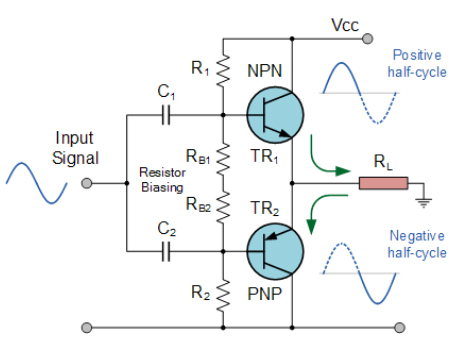
\includegraphics[width=8cm]{clase B.jpg}
\caption{Arreglo push-pull}
\end{figure}

En este punto la corriente de carga, se comparte entre los dos dispositivos, en medida cuando uno pierde intensidad el otro gana en parte esto, lo que hace que a lo largo del cilo las señales vayan reduciendo su voltaje y la corriente de salida, iguale a cero, en efecto esto se dupilca tanto la amplifiacion como la eficiencia del amplificador hasta un 70%.\\

Entrando en este punto, nos damos cuenta que la base de los transistores estan antifasicas, en este caso su emisor bajara en conexiones de corriente, a lo que el conector, se estara fluyendo de manera mas armonica, lo que hace que la corriente trabajada en un corte del colector y en cantidad igual y esto en vieceversa, siendo etapas del transoformador y la corriente entre los npn.\\

Siendo asi la condicion CC, en su funcionamieto estan pólarizados en el corte, por lo que el transistor solo conduce cuando la señal de entrada es mayor que la tension del emisor base, por lo tanto la entrada en cero da una salida cero y no cosume energia. Significando que el punto Q real de un amplificador tipo B trabaje en la linea de carga, en constante paso de corriente.\\

En otro punto de arreglo, en este caso sin transformador, lo que hace es tener una etapa de capacitancia, el cual haga su fluidez de corriente en pausas y e determiandos puntos, mas alta de un lado que de otro, trabajando en este caso en los transistores npn y pnp, en este caso es donde la efectividad se ve deteriorada por su efecto conocido, como distorsion cruzada.\\

\begin{figure}[hbtp]
\centering
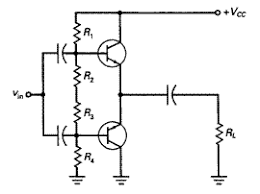
\includegraphics[width=6cm]{2.png}
\caption{Arreglo sin transformador}
\end{figure}


En este caso, como se hablo en las diferencia de los amplificadores de clase A y B, estos trabajan a una superacion de los 0.7v, en este punto para empezar a conducir, en este punto los amplificadores no estan predispuestos en un estado de funcionamiento en momento encendido. Esto es relevante , ya que en este caso el emisor del primer nucleo, trabaja en el nucleo del emisor del otro, en este caso, cuando uno es superado por su voltaje de entrada, empieza a trabajar en linea positiva, o en otro caso, cuando el primer transistor, se cierra el nucleo del otro transistor, empieza su labor, a lo que lo hace relevante al polo negativo del voltaje de amplificacion, en este punto los dos transistores no se detienen y comienzan a conducir en punto de cruce cero, inclusive si estos son pares coincidientes.\\

Conceptuando el cruce de voltaje en las salidas de los nucleos, en cada mitad de onda trabajando en los dos polos, se sabe que su area sera del mismo voltaje que seria los 0.7v, el resultado de esto aparte de estar conduciendo, es que estos se apaguen en forma simultanea.\\

Al trabajar con una sola fuente de coltaje es lo que genera los armonicos, a lo que la distorcion de su voltaje cruzado sera evidente, para acercarnos mas a una conceptualizacion mas simple, podemos guiarnos de dos fuentes de voltaje, para que cada nucelo trabaje, con su propia carga, y asi no generar disturbios entre corrientes, ni voltajes, y la potencia sea algo mucho mas eficiente, a la hora de empezar a hacer arreglos, de mayor alcance, y no solo en situaciones de amplifiacion. Pero en todo caso, no se recomienda ya que las uniones PN, se utilizan para proporcionar una adicion a los diodos. En todo caso, el simple hecho de que el Amplificador de clase B, trabaja a doble eficiencia, que los de clase A, en todo caso, dos remadores son mejor que uno.\\

\begin{figure}[hbtp]
\centering
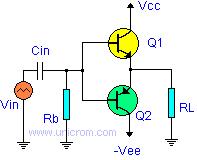
\includegraphics[width=6cm]{3.png}
\caption{Punto del NPN al PNP}
\end{figure}

En este caso, el circuito, puede trabajar de igual forma como el otro hablado, pero en este caso, las resistencias, tiene que hacer el trabajo, mas simplificado, ya que al solo colocar una sola resistencia, la entrega de voltaje sea mayor, liberando una mayor potencia, pero en us caso, un mayor ruido en su raea colocada. Haciendo esto, mas amplificado, pero a la vez mas eficiente, en algunos casos.\\

\subsection{Parametros:}

1- Entrega de voltaje en polos (positivo y negativo).\\
2- Superacion de los 0,7v, para su trabajo.\\
3- Entrega de potencia armonica al 0,2 por ciento.\\
4- Nucleos, enlazados entre PNP y NPN.\\
5- Energia disipada, por los nucleos.\\
6- Amplitud de onda, en un polo.\\ 
7- Corriente llegada a cero, cuando este, cruza su conexion con el emisor del segundo transistor.\\
8- Amplitud de onda incidente entre polos trabajados.\\
9- En una amplitud de onda reflejada en la entrada.\\
10-Amplitud de la onda es incidente en la salida.\\

\textbf{Referencias Bibliograficas:}\\
1- \url{http://tutorialesdeelectronicabasica.blogspot.com/2018/06/amplificador-de-clase-b-y-amplificador.html}\\
2- \url{https://www.youtube.com/watch?v=JSxEwDmtEQc}
\end{document}